\section{Signal and Noise}


\subsection{Material reference}
Content from TSE Book

\begin{itemize}
    \item Chapter 1 (Sections 1.1 and 1.2): overview of wireless communication
    \item Appendix A.1: Gaussian random variables
    \item Appendix A.2 (look through): signal detection in Gaussian noise
\end{itemize}


\noindent
Content from Haykin

\begin{itemize}
    \item Chapter 2.2 (page 8 to 14) 
    \item Chapter 2.8 (page 47 to 55)
\end{itemize}

\subsection{Fundamental Quantities and Signal Representation}

In wireless communication systems, voltage and power are closely related but conceptually distinct quantities. Voltage is an electrical potential difference measured in volts, while power represents the rate of energy transfer and is measured in watts. In resistive systems, power is proportional to the square of voltage, which is why power-based metrics dominate wireless analysis. Because received signal strengths can vary across many orders of magnitude, logarithmic units are used almost exclusively.

Wireless systems typically operate at high frequencies, ranging from kilohertz in legacy systems to gigahertz and beyond in modern cellular and satellite communications. High-frequency signals enable higher data rates and smaller antennas, but they are also more susceptible to attenuation, noise, and hardware imperfections. As frequency increases, the impact of thermal noise and propagation loss becomes more pronounced, making signal-to-noise ratio a central performance metric.

A received signal is always corrupted by noise, which is any unwanted disturbance that alters the signal. In most wireless systems, thermal noise dominates and is well modeled as additive white Gaussian noise. This noise is statistically independent of the transmitted signal and has a power that depends on temperature and bandwidth.

\subsection{Power in dBm and Logarithmic Representation}

Absolute power in wireless systems is often expressed in decibels relative to one milliwatt, denoted as dBm. The conversion from linear power to dBm is given by
\[
P_{\mathrm{dBm}} = 10 \log_{10}\left(\frac{P}{1\,\mathrm{mW}}\right).
\]
This logarithmic representation allows convenient comparison of power levels and simplifies link budget calculations. Power gains and losses, such as antenna gain or path loss, are expressed in decibels (dB), which represent ratios rather than absolute values.

A power gain expressed in decibels is defined as
\[
G_{\mathrm{dB}} = 10 \log_{10}\left(\frac{P_{\text{out}}}{P_{\text{in}}}\right),
\]
while absolute power is expressed in dBm. This distinction is important: dB values can be added and subtracted freely, while dBm represents an actual physical power level.

\section{Logarithmic Identities}

Logarithmic manipulation is fundamental in wireless communication analysis. For base-10 logarithms, the identities
\[
\log_{10}(ab) = \log_{10}(a) + \log_{10}(b), \quad
\log_{10}\left(\frac{a}{b}\right) = \log_{10}(a) - \log_{10}(b),
\]
and
\[
\log_{10}(a^n) = n \log_{10}(a)
\]
are used extensively when converting between linear and logarithmic domains. For base-2 logarithms, which arise naturally in information theory, the same identities hold with $\log_2$ replacing $\log_{10}$. Base-2 logarithms are particularly important when expressing data rates in bits per second.

\section{Signal Composition and Noise Model}

A signal in the time domain may be composed of multiple frequency components. For example,
\[
x(t) = 2\sin(t) + \sin(5t)
\]
represents the superposition of two sinusoidal signals with different amplitudes and frequencies. Such decompositions are fundamental to Fourier analysis and spectral interpretation.

In a noisy channel, the received signal is modeled as
\[
y(t) = x(t) + n(t),
\]
where $n(t)$ is additive noise. This model underpins most digital communication theory and allows performance analysis in terms of probability of error and signal-to-noise ratio.

\subsection{Filters and Frequency Selectivity}

Filters are used to control which frequency components of a signal are passed or attenuated. A low-pass filter allows frequencies below a cutoff frequency to pass, while attenuating higher frequencies. A high-pass filter does the opposite, passing high frequencies and suppressing low frequencies. Band-pass filters pass only a specific range of frequencies, while notch (band-stop) filters suppress a narrow frequency band while allowing others to pass.

\subsubsection{Filter Visualizations}

\begin{figure}[h]
\centering
\begin{tikzpicture}
\begin{axis}[
    width=10cm,
    height=5cm,
    xlabel={Frequency},
    ylabel={Magnitude},
    ymin=0, ymax=1.1,
    domain=0:10,
    samples=200,
    axis lines=left
]
\addplot[thick] {1/(1 + exp(3*(x-4)))};
\end{axis}
\end{tikzpicture}
\caption{Low-pass filter magnitude response}
\end{figure}

\begin{figure}[h]
\centering
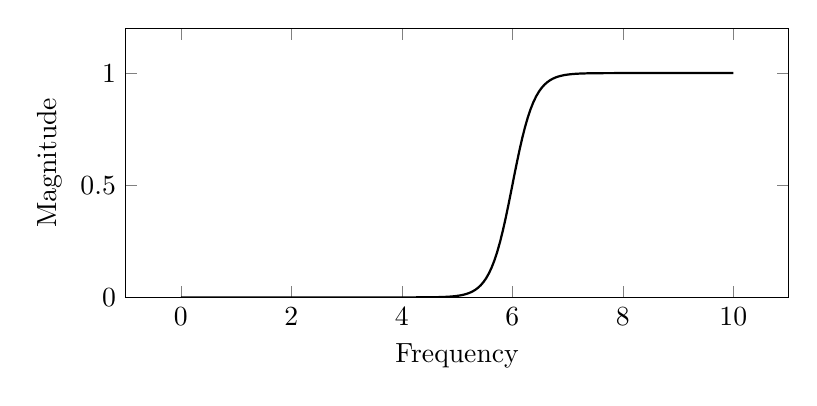
\begin{tikzpicture}
\begin{axis}[
    width=10cm,
    height=5cm,
    xlabel={Frequency},
    ylabel={Magnitude},
    ymin=0, ymax=1.2,
    domain=0:10,
    samples=200
]
\addplot[thick] {1/(1+exp(-5*(x-6)))}; 
\end{axis}
\end{tikzpicture}
\caption{High-pass filter magnitude response}
\end{figure}

\subsection{Link Budget and Measurement Instruments}

A link budget accounts for all gains and losses between the transmitter and receiver. The received power is given by
\[
P_{\mathrm{rx}} = P_{\mathrm{tx}} + G_{\mathrm{tx}} + G_{\mathrm{rx}} - L_{\mathrm{path}} - L_{\mathrm{other}},
\]
where all quantities are expressed in dB or dBm as appropriate. This equation provides an intuitive way to assess whether a communication link will close under given conditions.

Measurements are typically performed using a spectrum analyzer to observe signal power as a function of frequency, or a vector network analyzer to characterize frequency-dependent behavior such as gain, phase, and reflection. During lectures, readings in the range of 47–51 dBm were observed, indicating strong received signals or high reference levels depending on instrument configuration.

\subsection{Noise, Temperature, and Bandwidth}

Thermal noise power depends on temperature and bandwidth and is given in linear form by
\[
P_n = k_B T B,
\]
where $k_B$ is Boltzmann’s constant, $T$ is the absolute temperature in kelvin, and $B$ is the bandwidth in hertz. In logarithmic units, the noise power spectral density at room temperature is approximately $-174$ dBm/Hz. The total noise power in bandwidth $B$ is
\[
P_n = -174 + 10\log_{10}(B),
\]
with $B$ expressed in hertz.

Increasing bandwidth increases noise power but allows higher data rates. Narrow bandwidths provide finer spectral detail, while wider bandwidths are often easier to interpret and support higher throughput.

\subsection{Shannon Capacity and Energy Efficiency}

The maximum achievable data rate of a communication channel is given by Shannon’s capacity formula
\[
C = B \log_2(1 + \gamma),
\]
where $\gamma = \frac{P_s}{P_n}$ is the signal-to-noise ratio. This expression highlights diminishing returns: capacity grows logarithmically with SNR, meaning large power increases yield relatively small data rate improvements.

Energy efficiency is often expressed in bits per joule, or equivalently bits per watt-second. Communication systems are fundamentally limited by available power, and increasing spectral efficiency often comes at the cost of higher energy consumption.

\subsection{Modulation, BER, and Performance Metrics}

Information may be conveyed through amplitude, frequency, or phase modulation. Voice systems historically relied on analog modulation, while modern data systems use digital modulation schemes such as phase-shift keying. For PSK modulation, performance is often characterized using the ratio $E_b/N_0$, which relates the energy per bit to the noise spectral density.

The bit error rate (BER) quantifies the probability that a transmitted bit is incorrectly received. If $E = x - y$ denotes the error between transmitted and received bits, then the mean of $E$ corresponds to the BER. Experimental observations often show that distributions at power levels such as $-6$ dBm overlap significantly, indicating similar error behavior under those conditions.

\begin{figure}[h]
\centering
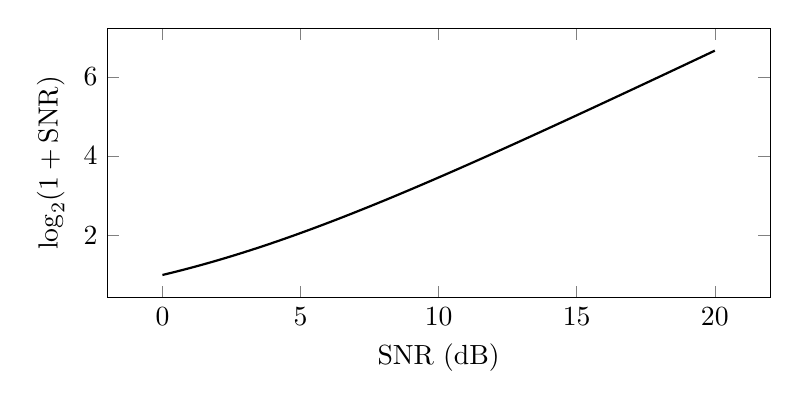
\begin{tikzpicture}
\begin{axis}[
    width=10cm,
    height=5cm,
    xlabel={SNR (dB)},
    ylabel={$\log_2(1+\mathrm{SNR})$},
    domain=0:20,
    samples=200
]
\addplot[thick] {ln(1 + 10^(x/10))/ln(2)};
\end{axis}
\end{tikzpicture}
\caption{Logarithmic growth of capacity with SNR}
\end{figure}


